\documentclass[../../main.tex]{subfiles}

\begin{document}

\begin{sloppypar}
Das nachfolgend dargestellte Diagramm skizziert das Verfahrensmodell, nach welchem die Umfragedaten verarbeitet werden. Es ist von oben nach unten, bzw. von links nach rechts zu lesen, siehe dazu auch die folgende Beschreibung:

\begin{itemize}
  \item Grundsätzlich wird zwischen Online-Umfrage und Interview unterschieden. 
  \item Der Fragentyp "`Offene Frage"' kommt sowohl in der Online-Umfrage \newline als auch in den Interviews vor.\footnote{Die Interviews beinhalten ausschliesslich offene Fragen.}
  \item In der linken Spalte folgen nach dem Fragentyp die Phasen Antworterfassung, \newline Nachbearbeitung und Auswertung. 
  \item Für jede Phase wird pro Fragetyp definiert wie die Antworten erfasst,\newline nachbearbeitet und ausgewertet werden.
\end{itemize}

Es ist ersichtlich, dass die Antworten auf die offenen Fragen aus der Online-Umfrage und die Antworten aus den Interviews für die Nachbearbeitungs- und Auswertungsphase zusammengeführt und verarbeitet werden.
\end{sloppypar}

\begin{figure}[H]
 \centering
    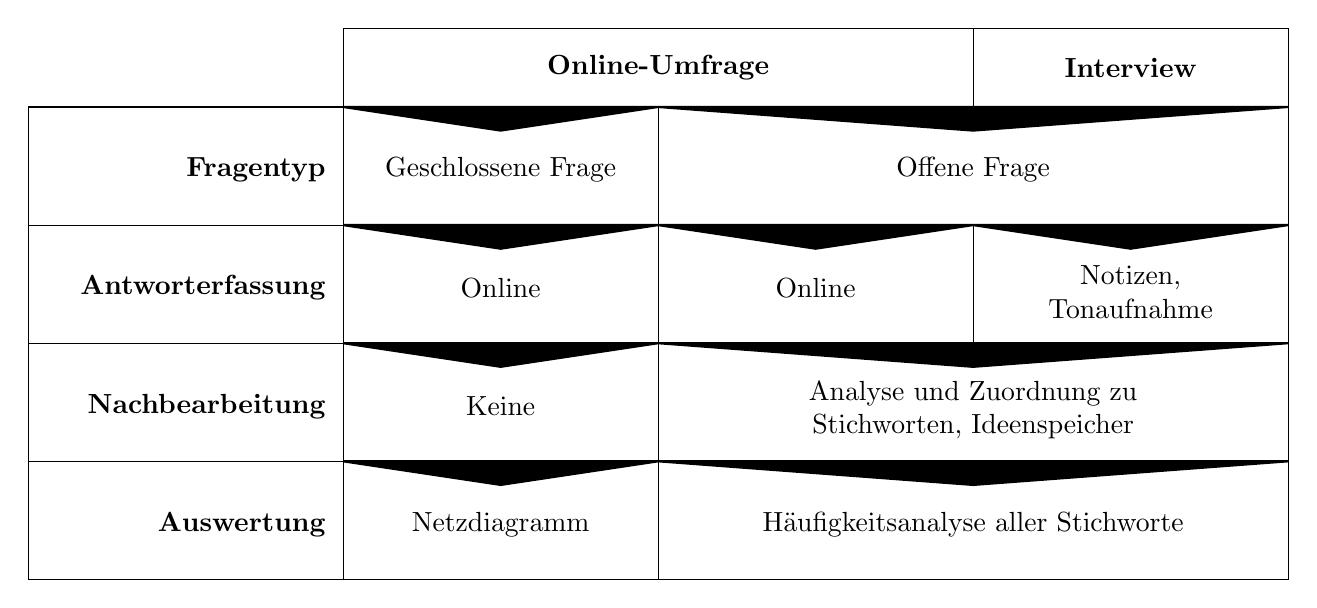
\begin{tikzpicture}

%% - Draw helping gridlines
%% - --------------------------------------

%\draw[step=2cm,gray,very thin] (0,0) grid (16,9);

%% - Draw table
%% - --------------------------------------

%% - surrounding box (biggest possible rectangle)

\draw[black, thin] (0,0) rectangle (16,6);

%% - vertical lines

\draw[black, thin] (4,0) -- (4,7);
\draw[black, thin] (8,0) -- (8,6);
\draw[black, thin] (16,6) -- (16,7);
\draw[black, thin] (12,6) -- (12,7);
\draw[black, thin] (12,3) -- (12,4.5);

%% - horizontal lines

\draw[black, thin] (4,7) -- (16,7);
\draw[black, thin] (0,4.5) -- (16,4.5);
\draw[black, thin] (0,3) -- (16,3);
\draw[black, thin] (0,1.5) -- (16,1.5);

%% - Draw arrows
%% - --------------------------------------

%% - geschlossene Frage
%% - --------------------------------------
\filldraw[color=black,fill=black, thick] (4,6) -- (8,6) -- (6,5.7) -- cycle;
%% - geschlossene Frage Online
%% - --------------------------------------
\filldraw[color=black,fill=black, thick] (4,4.5) -- (8,4.5) -- (6,4.2) -- cycle;
%% - geschlossene Frage Keine
%% - --------------------------------------
\filldraw[color=black,fill=black, thick] (4,3) -- (8,3) -- (6,2.7) -- cycle;
%% - geschlossene Frage Netzdiagramm
%% - --------------------------------------
\filldraw[color=black,fill=black, thick] (4,1.5) -- (8,1.5) -- (6,1.2) -- cycle;
%% - Offene Frage
%% - --------------------------------------
\filldraw[color=black,fill=black, thick] (8,6) -- (16,6) -- (12,5.7) -- cycle;
%% - Analyse & Zuordnung zu Stichworten
%% - --------------------------------------
\filldraw[color=black,fill=black, thick] (8,3) -- (16,3) -- (12,2.7) -- cycle;
%% - Frequenzanalyse aller Stichworte
%% - --------------------------------------
\filldraw[color=black,fill=black, thick] (8,1.5) -- (16,1.5) -- (12,1.2) -- cycle;
%% - Online
%% - --------------------------------------
\filldraw[color=black,fill=black, thick] (8,4.5) -- (12,4.5) -- (10,4.2) -- cycle;
%% - Notizen, Tonaufnahme
%% - --------------------------------------
\filldraw[color=black,fill=black, thick] (12,4.5) -- (16,4.5) -- (14,4.2) -- cycle;

%% - Draw Texts
%% - --------------------------------------

\node[draw,scale=1,shape=rectangle,draw=none,anchor=east,font=\bf] at (3.9,5.2) {Fragentyp};
\node[draw,scale=1,shape=rectangle,draw=none,anchor=east,font=\bf] at (3.9,3.7) {Antworterfassung};
\node[draw,scale=1,shape=rectangle,draw=none,anchor=east,font=\bf] at (3.9,2.2) {Nachbearbeitung};
\node[draw,scale=1,shape=rectangle,draw=none,anchor=east,font=\bf] at (3.9,0.7) {Auswertung};

\node[draw,scale=1,shape=rectangle,draw=none] at (6,5.2) {Geschlossene Frage};
\node[draw,scale=1,shape=rectangle,draw=none] at (6,3.7) {Online};
\node[draw,scale=1,shape=rectangle,draw=none] at (6,2.2) {Keine};
\node[draw,scale=1,shape=rectangle,draw=none] at (6,0.7) {Netzdiagramm};

\node[draw,scale=1,shape=rectangle,draw=none] at (12,5.2) {Offene Frage};
\node[draw,scale=1,shape=rectangle,draw=none,text width=7cm,align=center] at (12,2.15) {Analyse und Zuordnung zu Stichworten, Ideenspeicher};
\node[draw,scale=1,shape=rectangle,draw=none] at (12,0.7) {Häufigkeitsanalyse aller Stichworte};

\node[draw,scale=1,shape=rectangle,draw=none] at (10,3.7) {Online};
\node[draw,scale=1,shape=rectangle,draw=none,text width=3cm,align=center] at (14,3.65) {Notizen, Tonaufnahme};

\node[draw,scale=1,shape=rectangle,draw=none,font=\bf] at (8,6.5) {Online-Umfrage};
\node[draw,scale=1,shape=rectangle,draw=none,font=\bf] at (14,6.5) {Interview};

\end{tikzpicture}

 \caption{Verfahrensmodell für Auswertung der Online-Umfrage und Interviews}
 \label{Allgemeines Vorgehen}
\end{figure}

\end{document}
